\title{\large e1-6 Proton Identification}
\maketitle

\abstract{This chapter describes the proton identification for the e1-6 data.
The candidate protons are all the events containing at least one positive time-based track, after the electron identification.
The cuts are based on the candidate's reconstructed momentum and its signals on
the Time of Flight (TOF)\cite{bib:ftof}. The cuts are sector-dependent.}

\tableofcontents

\section{Proton identification}

The purpose of this study is the proper identification of the
scattered protons. The CLAS timing resolution decreases as the
particles momentum increases. It is problematic to properly identify
charged particles with the timing  information alone at very large (greater than $3, 4$ GeV) momentum.
The goal of this analysis is to make the best possible selection of protons, while keeping
in mind that further refinements based on individual reactions kinematics will be necessary.



\subsection{CLAS Timing}
\label{sec:clas_timing}


During the event reconstruction the momentum of a track is calculated 
with the tracking procedure \cite{bib:tracking}. To determine its speed $\beta$,
the start time $T_0$ is calculated as
\begin{equation}
 T_0 = T_{el} - \frac{\ell}{c} - \frac{z-z_0}{c}
\end{equation}
where $T_{el}$ is the electron time from TOF measurement, $\ell$ is the
path length of the electron track from the vertex to its TOF hit, $c$ is
the speed of light, $z$ is the z-component of the event vertex and $z_0$ 
is the $z$ position of the center of the 
target\footnote{For this experiment $z_0 = -4$ cm.}. $T_0$ is then used 
as the reference for all the remaining tracks in the event. The track speed $\beta$ 
is calculated as:
\begin{equation}
 \beta = \frac{v}{\it c} = \frac{1}{c} \frac{\ell}{T-T_0}
\end{equation}
where $\ell$ is the track path length from the target and $T$ its TOF time.
In  Fig.\ref{fig:beta_vs_mom} is plotted $\beta$ versus momentum for the all the 
particles after the electron particle ID. One can clearly see bands corresponding 
to pions, kaons, protons, deuterons.


\begin{figure}[h]
  \centering
		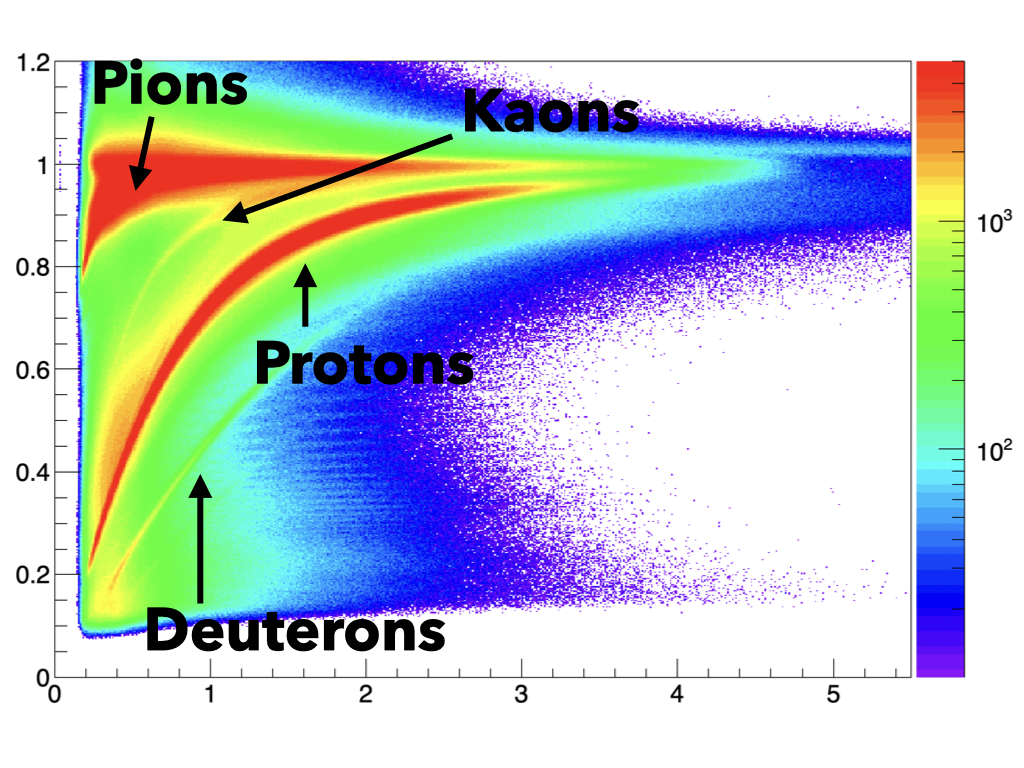
\includegraphics[width=0.75\textwidth ]{img/beta_vs_mom}
		\caption{ $\beta$ versus momentum for positive particles in e1-6 running period. Bands
                    corresponding to pions, kaons, protons and deuterons are visible.}
 		\label{fig:beta_vs_mom}
\end{figure}

\subsection{$\Delta T$ cut}
\label{sec:clas_timing}

For this analysis every positive track (determined by its curvature in the torus field) 
is a {\it proton candidate}.

The difference $\Delta T$ between the time calculated using
the candidates's momentum (assuming it is a proton) and its actual TOF time $T$ 
should peak at zero for protons:
\begin{equation}
 \label{eq:protondt}
  \Delta T = \frac{\ell}{\beta'} + T_{0} - T (\sim0 )
\end{equation}
where $\beta' = \sqrt{ p^2 /( M_P^2 + p^2 ) }$ is the speed of the track calculated from its
momentum and $M_P$ is the proton mass. 
A plot of $\Delta T$ versus momentum for Sector 1 is shown in 
Fig.\ref{fig:dt_vs_mom}. The distribution is sliced along $\Delta T$ and each slide is fitted
with $2$ Gaussians + $2^{nd}$ order polynomial function to calculate the mean 
positions $\mu$ and sigmas $\sigma$ of the proton and pions/kaons signals. 
The proton's $\mu$ and $\sigma$ are then fitted with a $5^{th}$-order polynomial. 
An example of $\mu$ fit is also shown in 
Figures \ref{fig:dt_vs_mom} and \ref{fig:dt_vs_mom_all_sectors}.

At low momentum the protons are well separated.  The pions distribution 
start to contaminate the protons when
$\mu_{P} + 3\sigma_{P} < \mu_{\pi} - 3\sigma_{\pi}$;  in that case 
$(\mu_{\pi} - 3\sigma_{\pi} - \mu_{P})/3$ is used as the signal $\sigma$ instead of $\sigma_{P}$.
In Fig.\ref{fig:dt_vs_mom_all_sectors} the cuts for all sectors are shown. 

Two quantities normally used to monitor the quality of the charged particles
selection are $\beta$ and the TOF Mass $M_{TOF}^2$:
$$
 M_{TOF}^2 = \frac{p^2(1-\beta^2)}{\beta^2}
$$
Both $\beta$ and $M_{TOF}^2$ versus momentum are shown for sector 5 in 
Fig.\ref{fig:mass_beta_vs_p_sect5}. The $M_{TOF}^2$ was initially considered
to perform this identification. However, when sliced, the corresponding
1-dimensional plots could not resolve the protons and kaons/pions signal 
as well as $\Delta T$ can.

The value of the $\mu$ and $\sigma$ parameters used are listed in sec\ref{sec:dtp_parameters}.




\subsubsection{Cut parameters}\label{sec:dtp_parameters}
$$
f(p) = a + bp + cp^2 + dp^3 + ep^4 + fp^5
$$
\begin{verbatim}

           S1           S2           S3           S4          S5            S6
mean:
a:      -0.9113    -0.655048    -0.904261    -0.709094    -0.724329    -0.418643
b:      2.98931      1.38425      1.76954     0.591925      4.06097     0.781139
c:     -4.09545     -2.10418      -1.9409     0.272274      -5.8547    -0.943656
d:      2.19893       1.2356     0.948967    -0.454383      3.18819     0.501819
e:    -0.495131    -0.290715    -0.194741     0.158209    -0.720678    -0.117491
f:    0.0389196    0.0232255    0.0136907   -0.0165409    0.0568144   0.00959472

sigma 
a:      6.16714      6.60215      5.87269      5.90242      5.96331      5.99657
b:     -12.1628     -14.4183     -10.6575     -11.7175     -12.2304     -12.4064
c:      9.86015      12.6391      8.00035      9.75136       10.391        10.69
d:     -3.74511     -5.02972     -2.86622     -3.90726     -4.04935     -4.35567
e:     0.679294     0.926557     0.497855     0.750446     0.737621     0.835659
f:   -0.0470408   -0.0639353    -0.033369   -0.0545215   -0.0505353   -0.0600134

\end{verbatim}

\clearpage\newpage

\begin{figure}[ht]
  \centering
		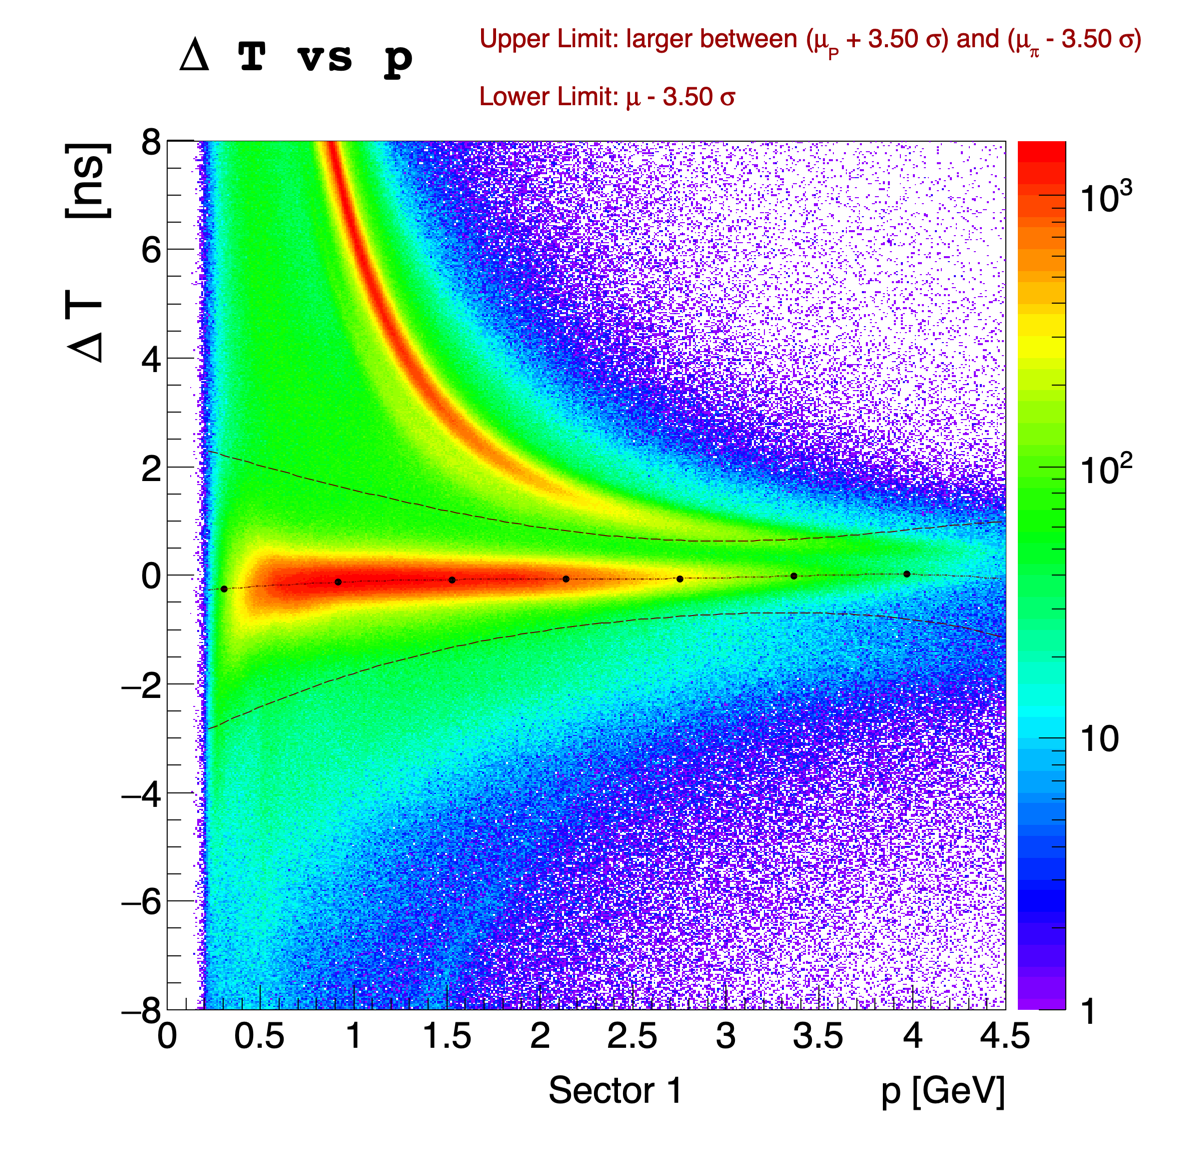
\includegraphics[width=0.88\textwidth ]{img/dist-dtfit_sector-1}
		
		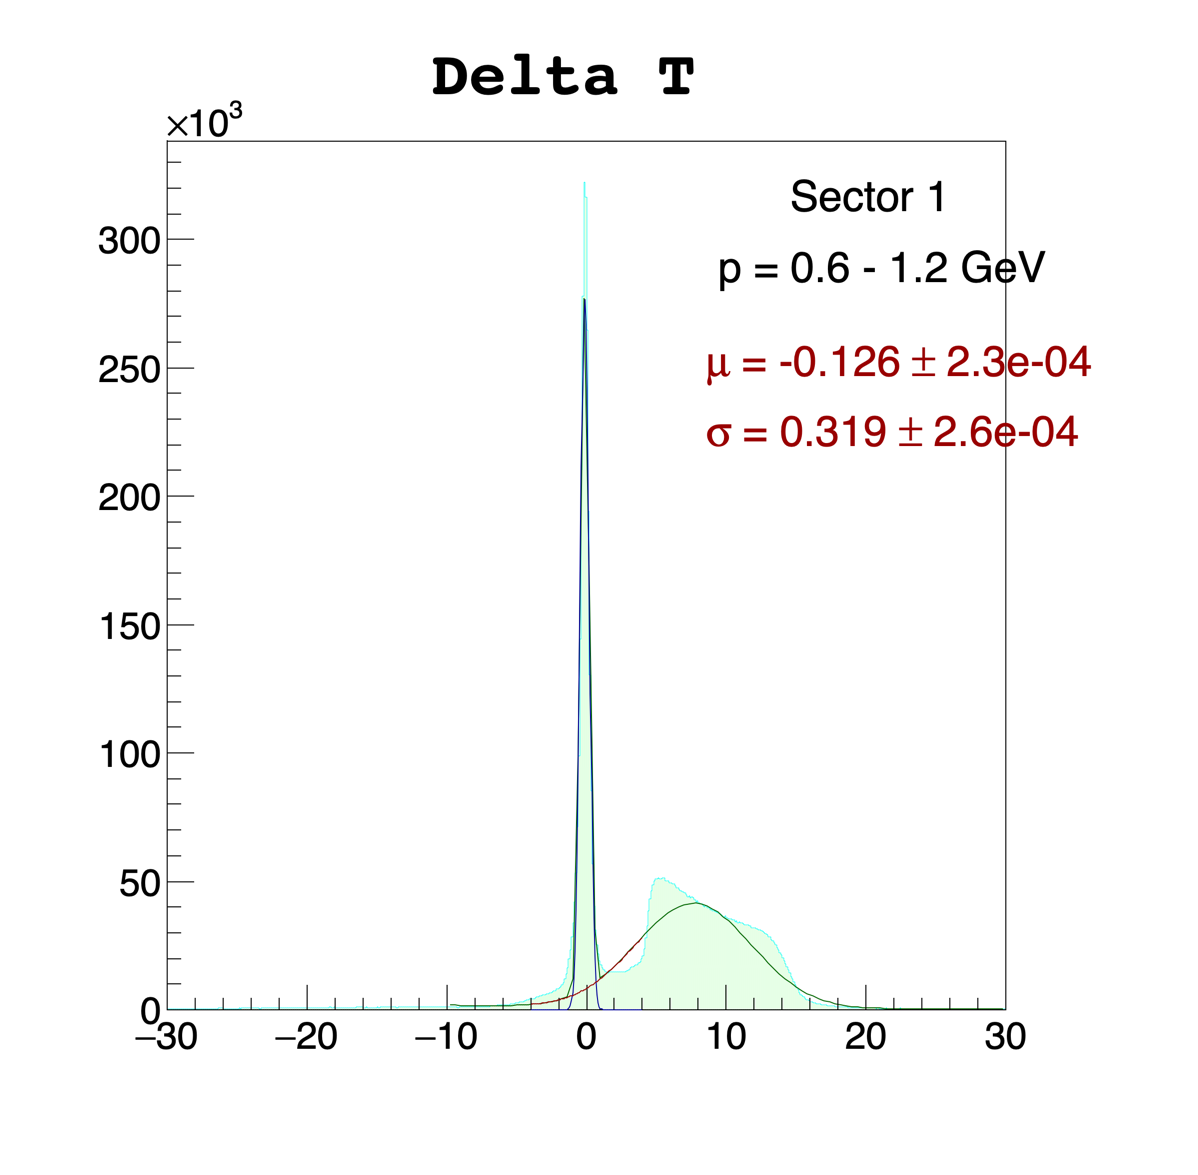
\includegraphics[width=0.47\textwidth]{img/slice-2_sector-1}
		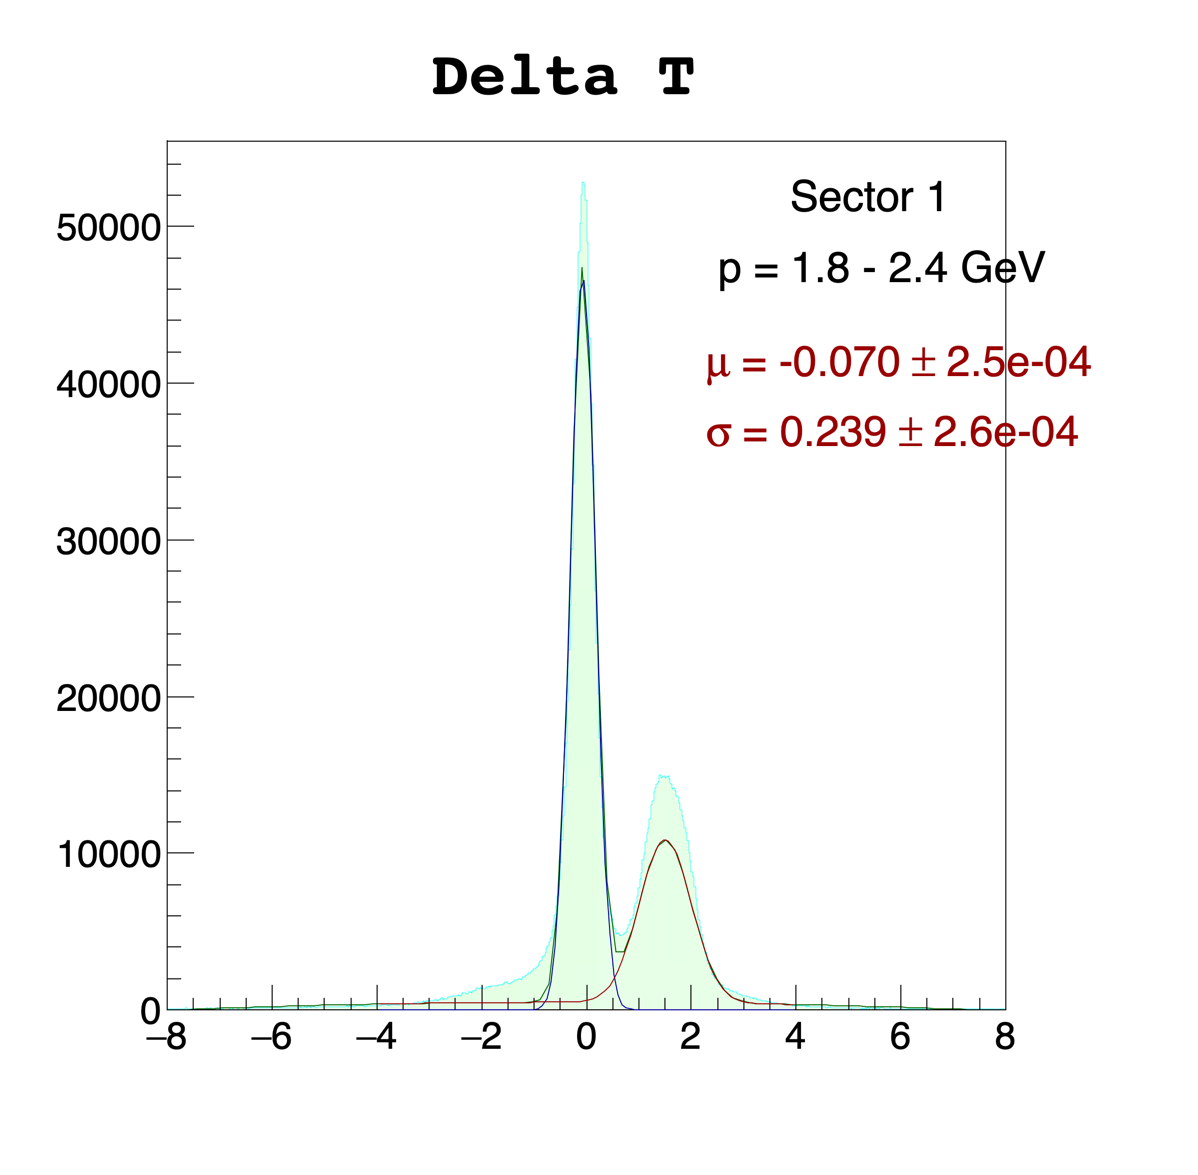
\includegraphics[width=0.47\textwidth]{img/slice-4_sector-1}
		
		\caption{$\Delta T$ versus momentum and slices at different momentum.
					At low momentum the proton signal is well separated
					from kaons and pions, so we include everything up to
					$3\sigma$ from the pion/kaons signal. At high momentum 
					kinematic constrains for exclusive channels will be necessary.
					The colors are as follows: blue: proton signal (gaussian).
					Red: pion signal (gaussian) + background ($2^{nd}$ order 
					polynomial). Dark green: total fit function.}
 		\label{fig:dt_vs_mom}
\end{figure}

\clearpage\newpage

\begin{figure}[ht]
	\centering
		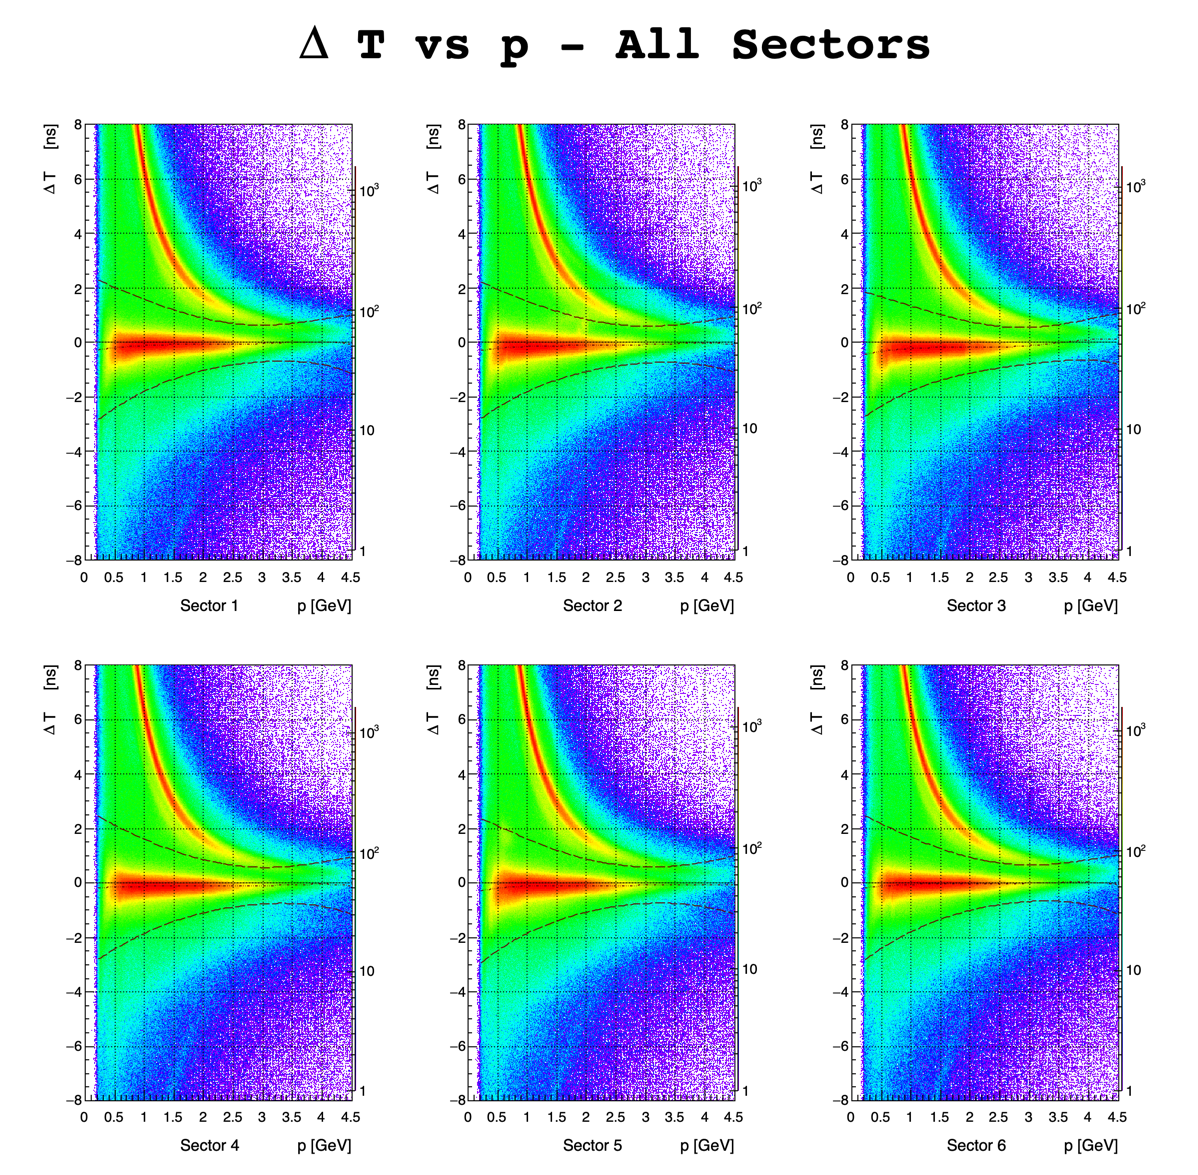
\includegraphics[width=0.95\textwidth]{img/dist-dtfit_sector-all}
		\caption{$\Delta T$ versus momentum cuts in all sectors. Plot grids
					emphasize the differences between sectors.}
		\label{fig:dt_vs_mom_all_sectors}
\end{figure}

\clearpage\newpage

\begin{figure}[ht]
	\centering
		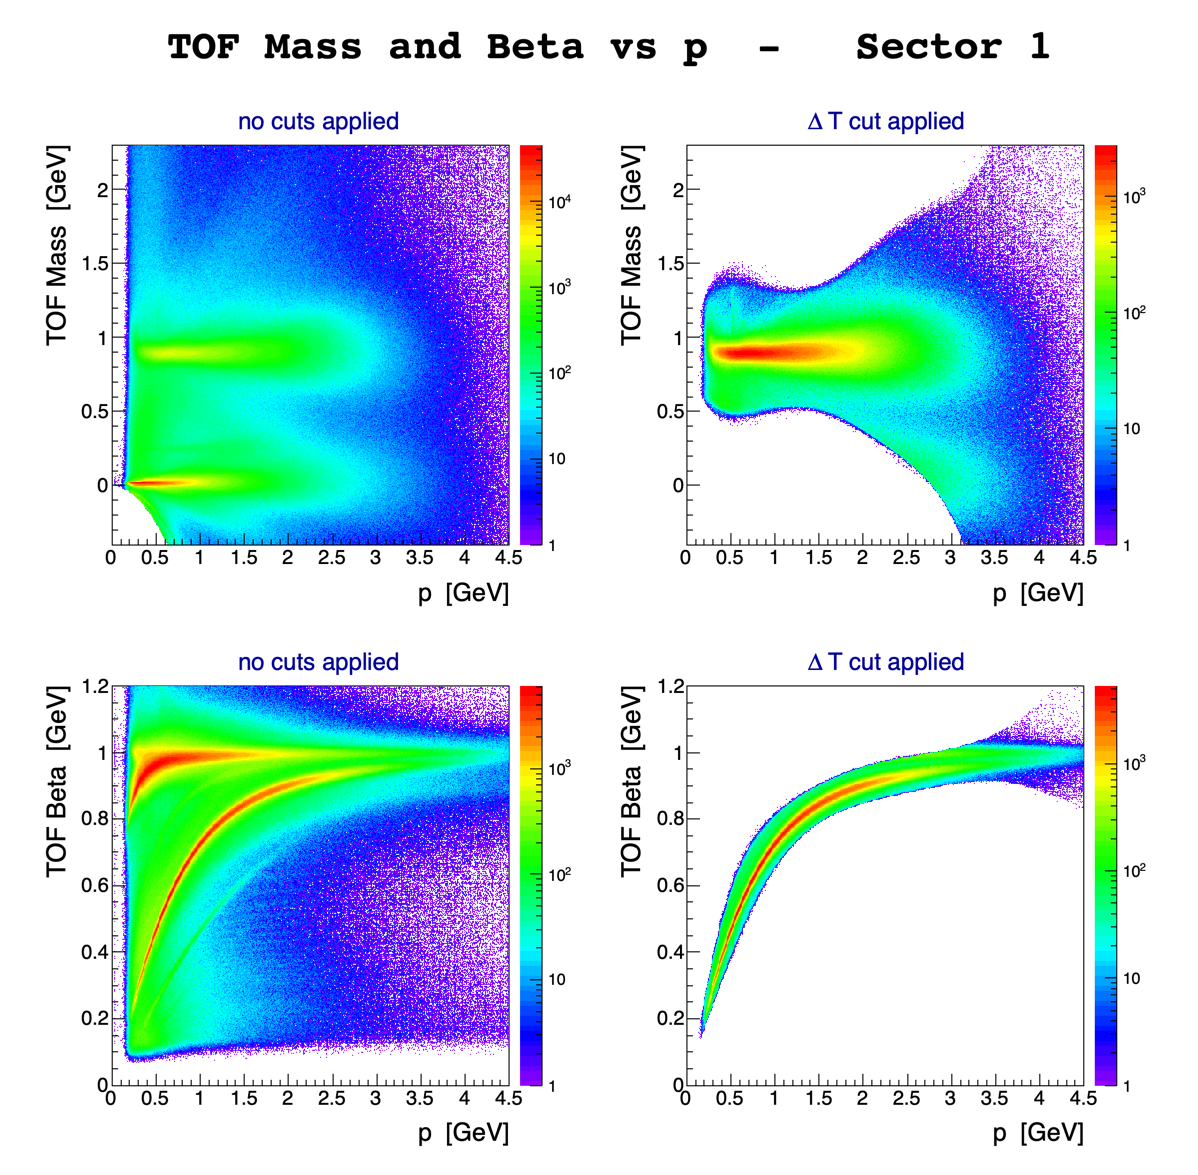
\includegraphics[width=0.95\textwidth]{img/dist-massandbeta_sector-1}
		\caption{Left: $\beta$ and $M_{TOF}^2$ versus momentum for positive
					tracks with no cut applied. Right: the same quantities with the
					$\Delta T$ cut applied.}
		\label{fig:mass_beta_vs_p_sect5}
\end{figure}

The complete set of plots can be found on the web \cite{bib:pi0_resonance_id_proton}.


\clearpage








\begin{thebibliography}{mybib}
    \bibitem{bib:ftof}                   {E.S. Smith et al.}, The Time-of-Flight System for CLAS,                                      {\textit Nucl. Inst. and Meth. A 432, 265 (1999)}
    \bibitem{bib:tracking}               {B. Niczyporuk},     \href{http://www.jlab.org/Hall-B/notes/clas_notes91/note91-001.pdf}      {\textit CLAS-NOTE 91 - 001}
    \bibitem{bib:pi0_resonance_id_proton} {M.Ungaro},         \href{https://maureeungaro.github.io/home/meson/pi0_resonance/proton_id} {\textit Proton identification for single $\pi^0$ elctroproduction in the first and second resonance regions}
\end{thebibliography}


\end{document}








